
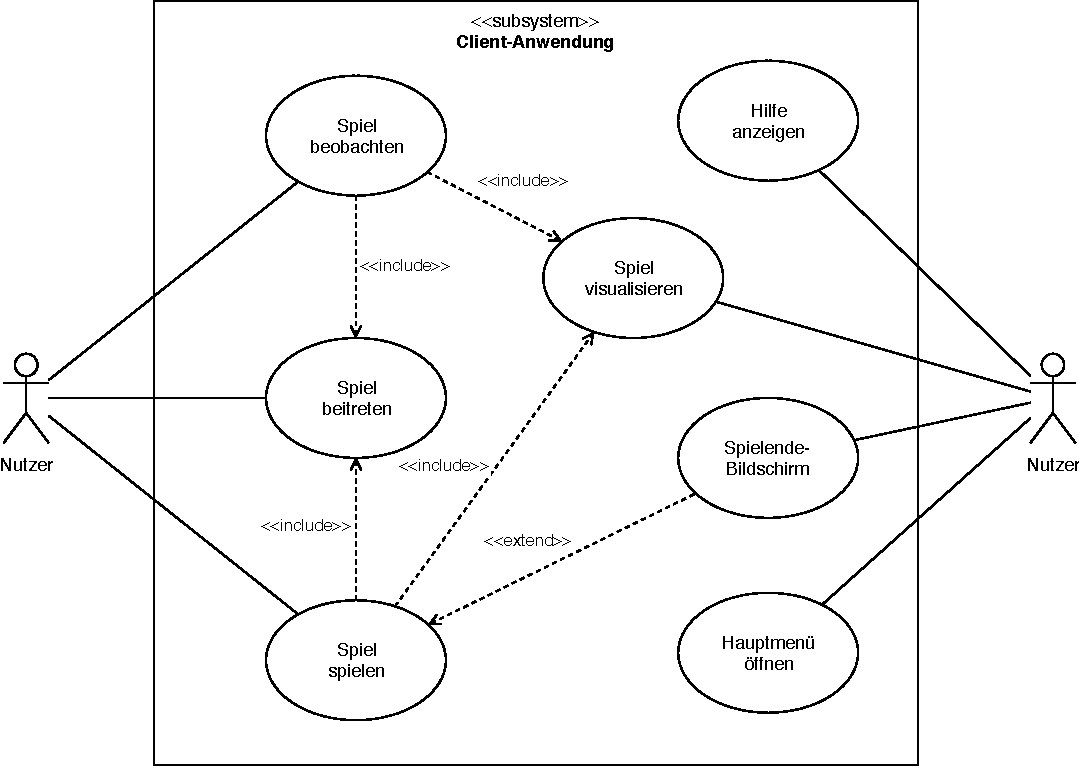
\includepdf[pages=-, scale=0.8, pagecommand={\subsection{Anwendungsfälle}\subsubsection{Client}Anwendungsfälle der Client-Anwendung. Der Anwendungsfall \glqq{}Spiel spielen\grqq{} wird unter \ref{ssec:Partie}~ konkretisiert. Hinweis: Der zweite Akteur wurde nur aus Übersichtlichkeitsgründen hinzugefügt und stellt keinen zweiten Nutzer dar.}]{../Meilenstein02/images/AFD_Client.pdf}

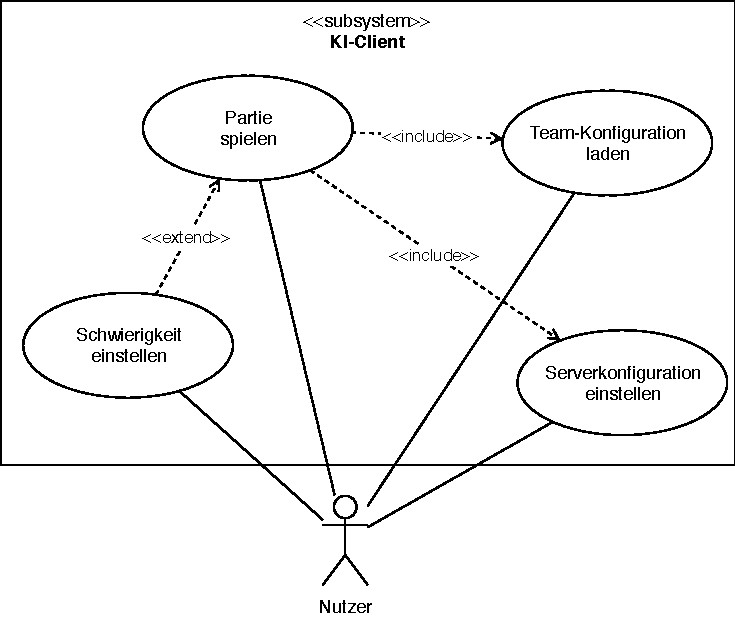
\includepdf[pages=-, scale=0.8, pagecommand={\subsubsection{KI-Client}Anwendungsfälle des KI-Clients. Diese Anwendung verbindet sich mit einem Server und simuliert mithilfe einer zuvor konfigurierten KI einen menschlichen Gegenspieler. Der Anwendungsfall \glqq{}Spiel spielen\grqq{} wird unter \ref{ssec:Partie}~ konkretisiert.}]{../Meilenstein02/images/AFD_KIClient.pdf}

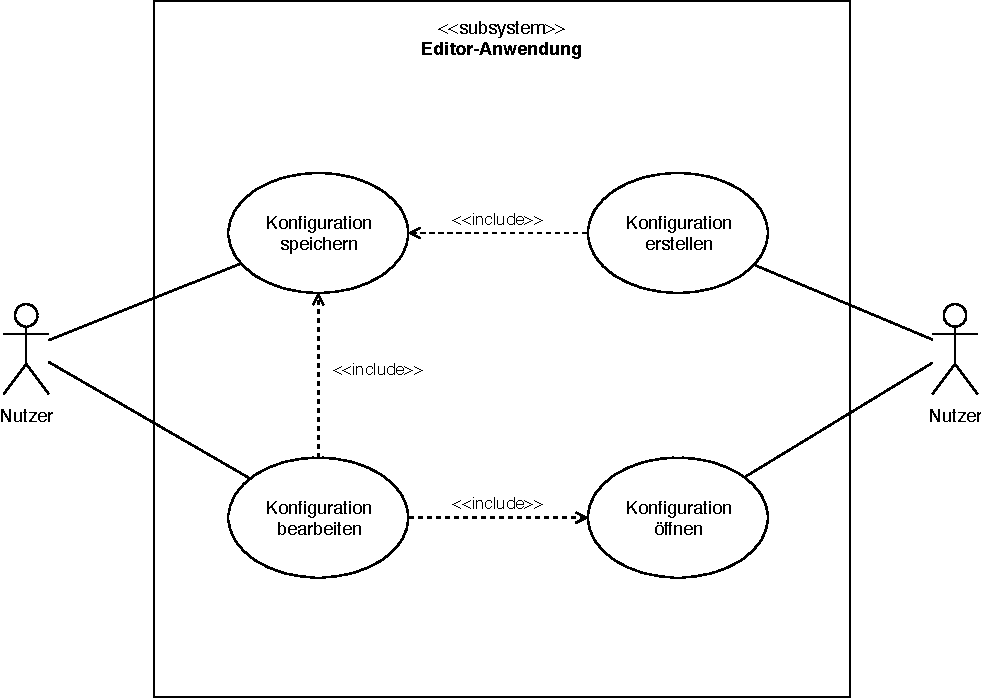
\includepdf[pages=-, scale=0.8, pagecommand={\subsubsection{Editor}Anwendungsfälle der Editor-Anwendung. Der zweite Akteur wurde nur aus Übersichtlichkeitsgründen hinzugefügt und stellt keinen zweiten Nutzer dar.}]{../Meilenstein02/images/AFD_Editor.pdf}
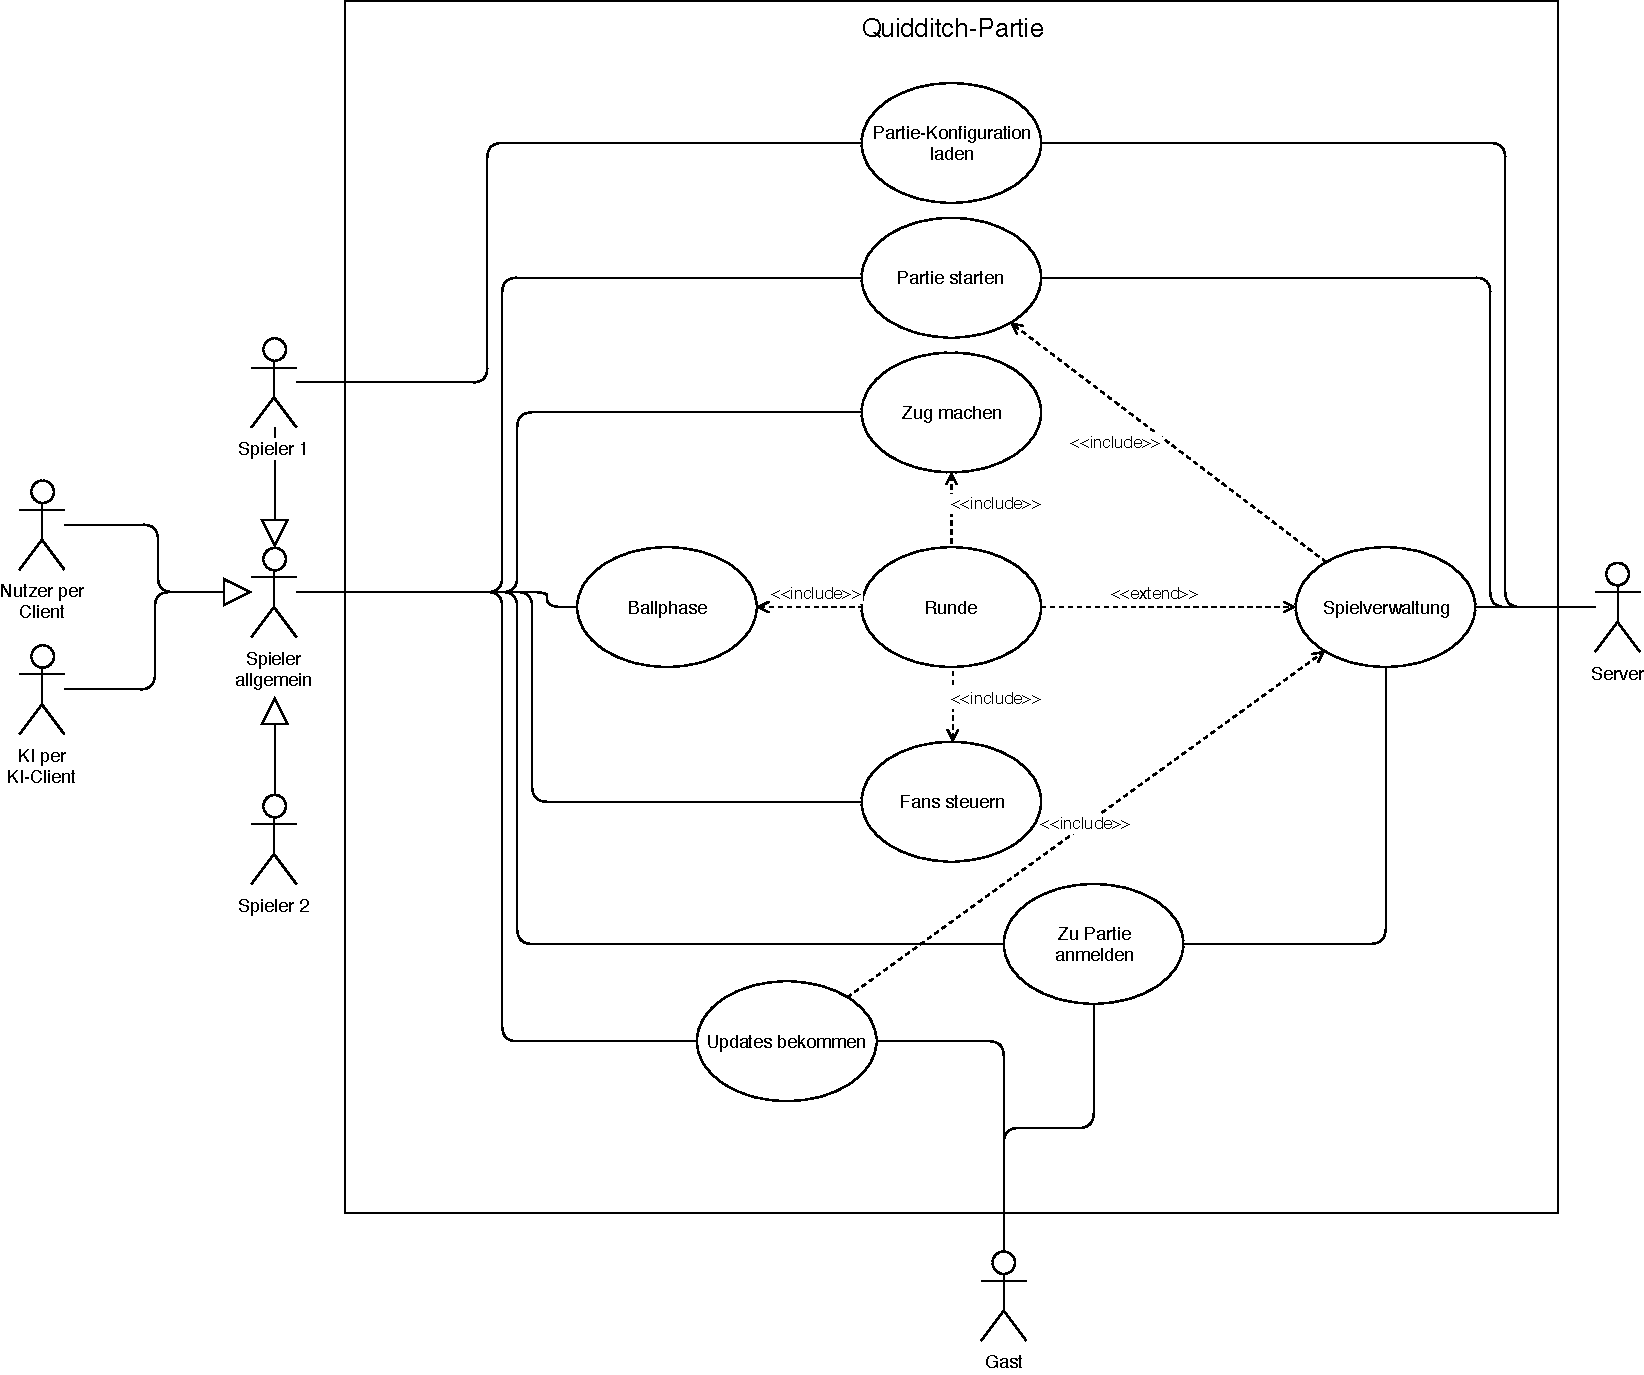
\includepdf[pages=-, scale=0.8, pagecommand={\subsubsection{Partie}\label{ssec:Partie}Mögliche Anwendungsfälle, die während einer Partie auftreten. Die Runde stellt einen abstrakten Anwendungsfall dar, der sich aus den einzelenen Phasen einer Runde zusammensetzt.}]{../Meilenstein02/images/AFD_Party.pdf}


\subsection{Zuordnung der Anforderungen zu Anwendungsfällen}
Hier wird aufgelistet, welche funktionalen Anforderungen (siehe \ref{FAs}) von den jeweiligen Anwendungsfällen abgedeckt werden.
\subsubsection{Hauptmenü öffnen}
FA60

\subsubsection{Hilfe anzeigen}
FA65

\subsubsection{Spielende-Bildschirm}
FA49,
FA62

\subsubsection{Spiel visualisieren}
FA1,
FA2, 
FA3, 
FA4, 
FA5, 
FA6, 
FA64

\subsubsection{Spiel beobachten}
FA55,
FA66

\subsubsection{Spiel beitreten}
FA55,
FA61

\subsubsection{Spiel spielen}
FA14, 
FA15, 
FA16, 
FA17, 
FA18, 
FA19, 
FA20, 
FA55, 
FA67,
FA68, 
FA69,
FA73 

\subsubsection{Serverkonfiguration einstellen}
FA74 

\subsubsection{Team-Konfiguration laden}
FA75 

\subsubsection{Konfiguration erstellen}
FA14,
FA15, 
FA53, 
FA54, 
FA71

\subsubsection{Konfiguration speichern}
FA14,
FA15, 
FA53, 
FA54, 
FA71

\subsubsection{Konfiguration bearbeiten}
FA14,
FA15, 
FA53, 
FA54, 
FA70, 
FA72

\subsubsection{Konfiguration öffnen}
FA14,
FA15, 
FA53, 
FA54, 
FA63

\subsubsection{Team-Konfiguration laden}
FA14,
FA15, 
FA54, 
FA55, 
FA63

\subsubsection{Partie starten}
FA50,
FA51, 
FA55

\subsubsection{Zug machen}
FA8,
FA21, 
FA22, 
FA24, 
FA26, 
FA27, 
FA28, 
FA29, 
FA30, 
FA37, 
FA38, 
FA39, 
FA40, 
FA41, 
FA42, 
FA46, 
FA55

\subsubsection{Runde}
FA10,
FA11, 
FA12, 
FA13, 
FA25, 
FA44, 
FA55

\subsubsection{Ballphase}
FA10,
FA11, 
FA12, 
FA13, 
FA29, 
FA45, 
FA55 

\subsubsection{Fans steuern}
FA31,
FA32, 
FA33, 
FA34, 
FA35, 
FA47, 
FA55 

\subsubsection{Spielverwaltung}
FA1,
FA2, 
FA3, 
FA4, 
FA5, 
FA6, 
FA7, 
FA9, 
FA23, 
FA30, 
FA36, 
FA43, 
FA48, 
FA49, 
FA52, 
FA53, 
FA54, 
FA56, 
FA58, 
FA59 

\subsubsection{Updates bekommen}
FA55

\subsubsection{Zu Partie anmelden}
FA55

\subsubsection{Partie-Konfiguration laden}
FA53,
FA57

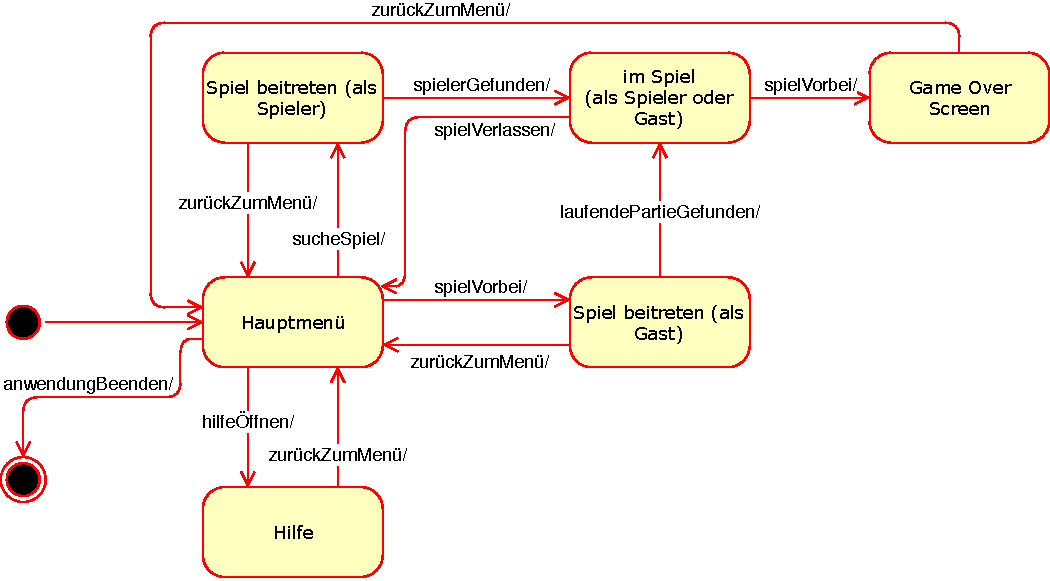
\includepdf[pages=-, scale=0.8, pagecommand={\subsection{Abläufe im System}\subsubsection{State-Machine Clientanwendung} Zustandsdiagramm für die verschiedenen Ansichten der Client-Anwendung.}]{../Meilenstein02/images/Client_SM.pdf}

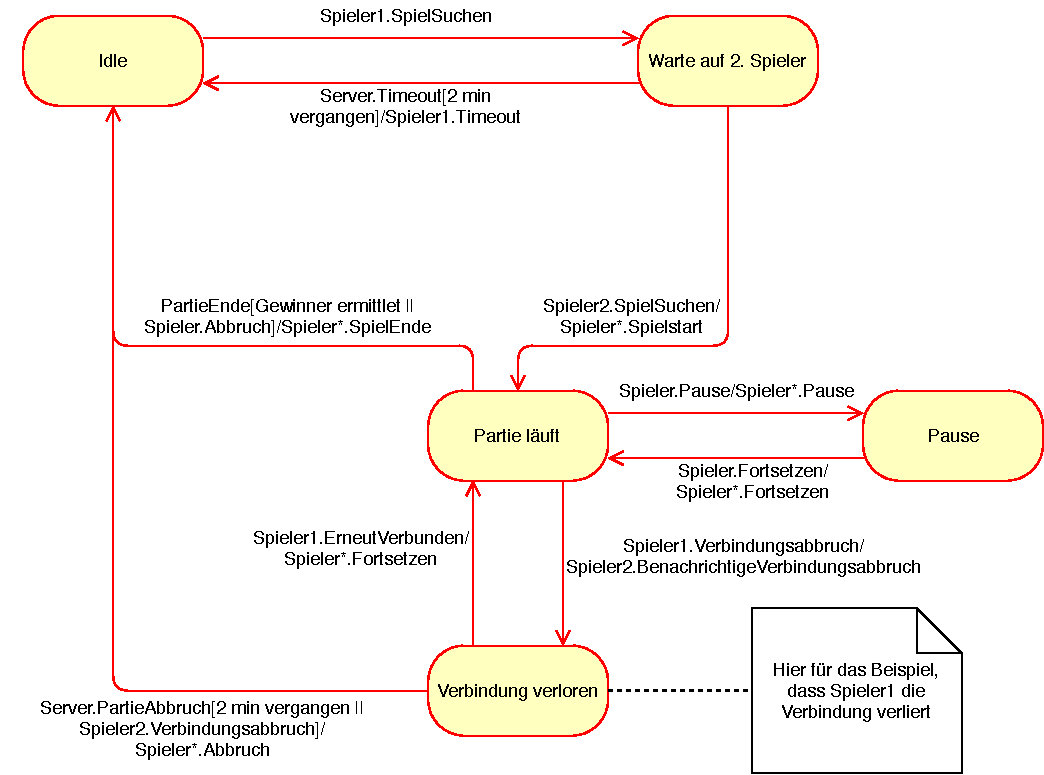
\includepdf[pages=-, scale=0.8, pagecommand={\subsubsection{State-Machine Partie Server} Zustandsdiagramm des Servers für eine komplette Partie, inklusive Anmeldung der Spieler und eventuelle Verbindungsabbrüche.}]{../Meilenstein02/images/SM_Server.pdf}

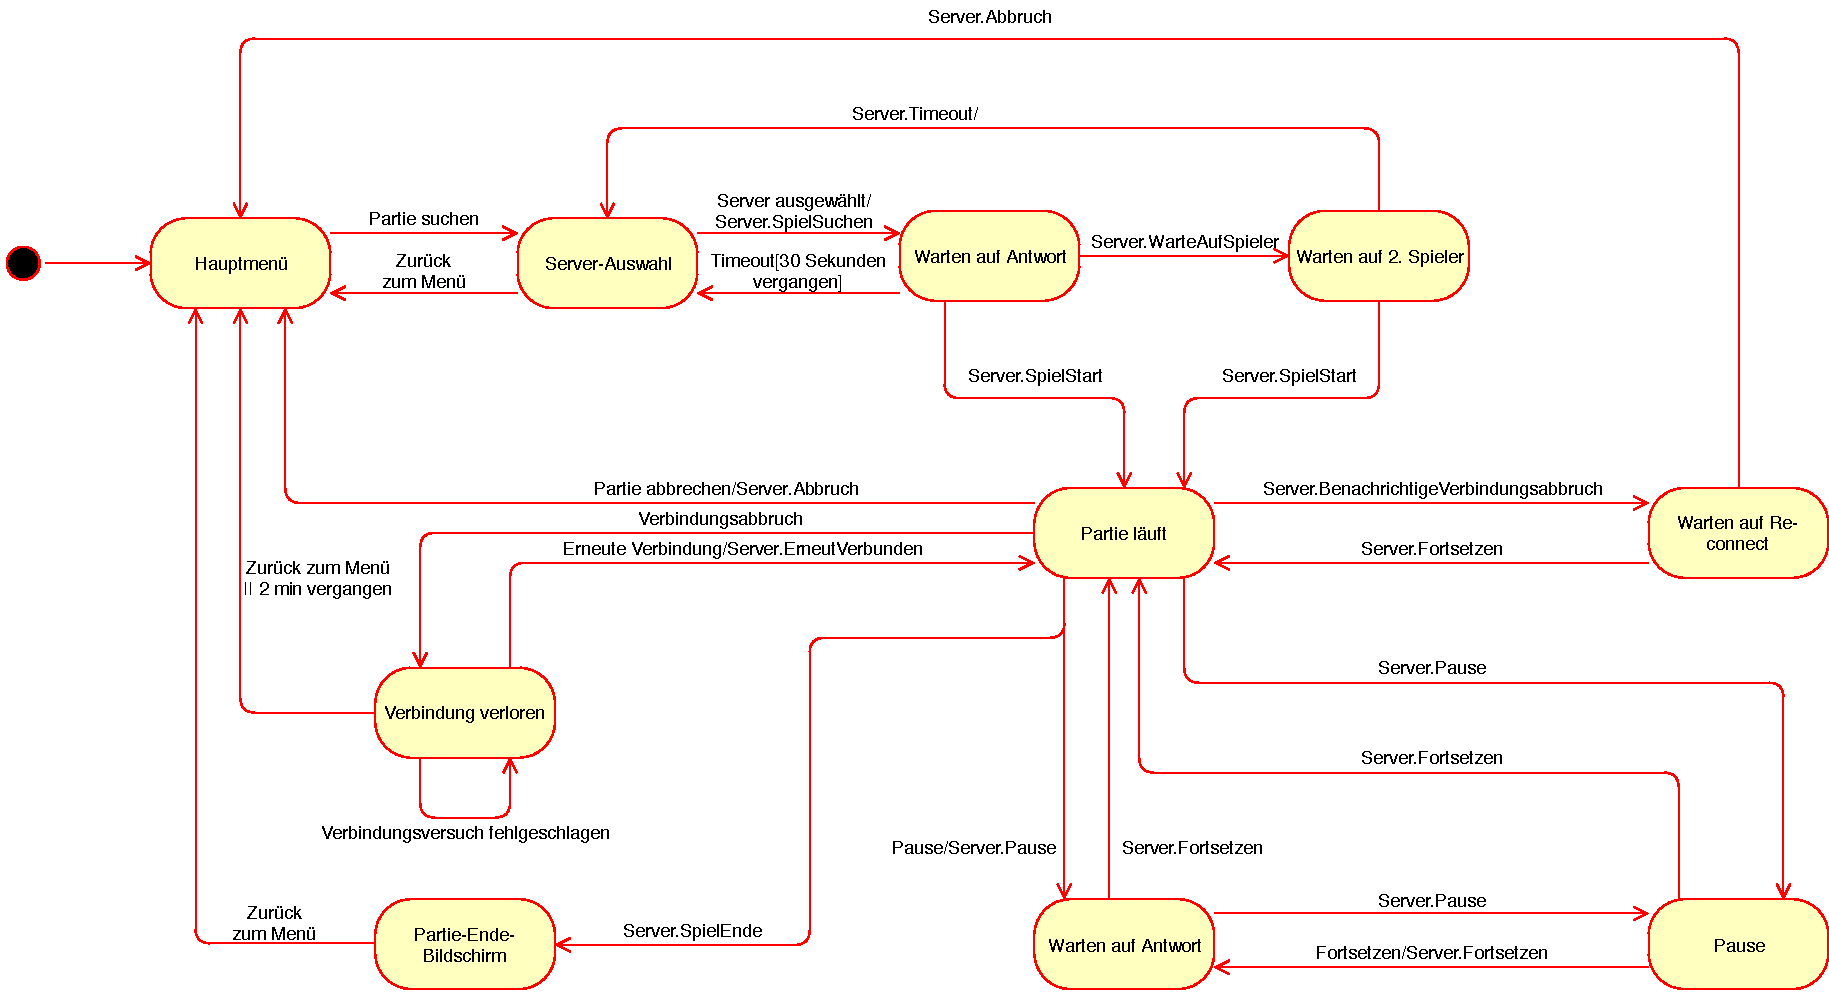
\includepdf[pages=-, scale=0.9, pagecommand={\subsubsection{State-Machine Partie Client}Zustandsdiagramm der Client-Anwendung für eine komplette Partie.}]{../Meilenstein02/images/SM_ClientAnmelden.pdf}

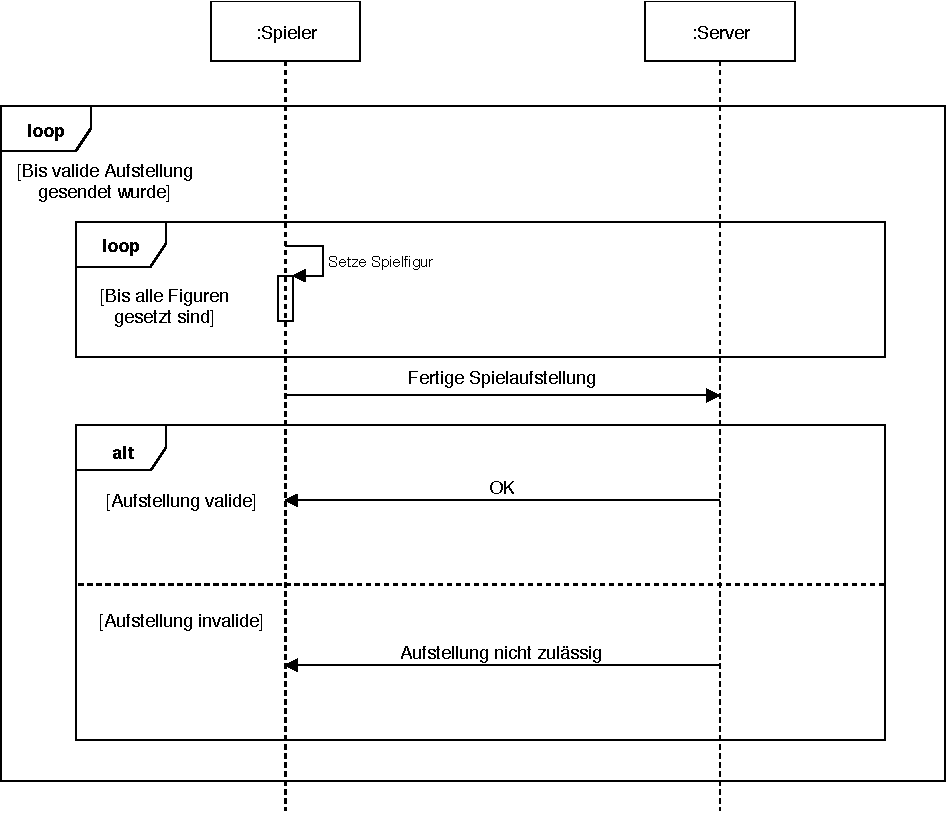
\includepdf[pages=-, scale=0.8, pagecommand={\subsubsection{Sequenzdiagramm Spielaufstellung}Kommunikation zwischen Spieler und Server während der Spielaufstellungsphase.}]{../Meilenstein02/images/SD_Spielaufstellung.pdf}

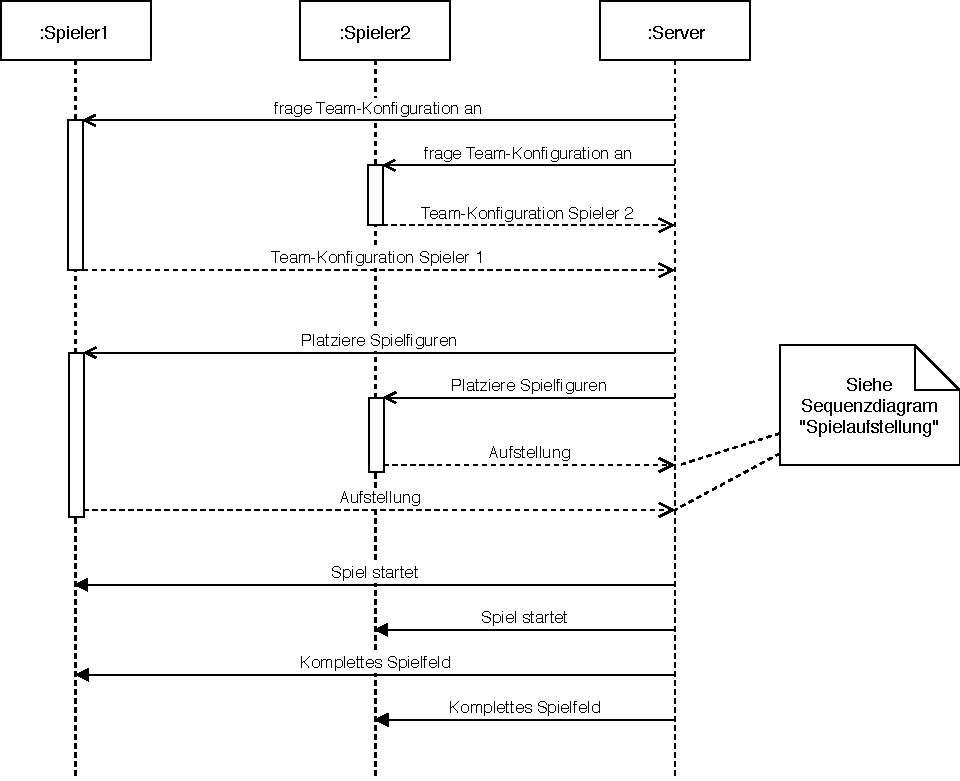
\includepdf[pages=-, scale=0.8, pagecommand={\subsubsection{Sequenzdiagramm Spielvorbereitung}Nachrichtenaustausch zwischen Server und den Spielern während der Vorbereitung auf die Partie.}]{../Meilenstein02/images/SD_Spielvorbereitung.pdf}
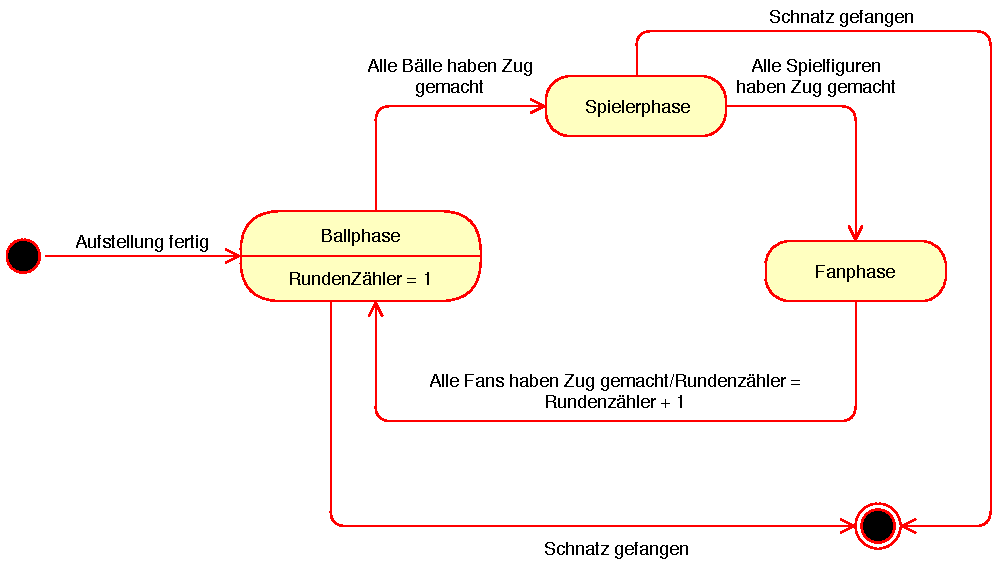
\includepdf[pages=-, scale=0.8, pagecommand={\subsubsection{State-Machine Rundenablauf}Ablauf der Spielphasen im Spiel}]{../Meilenstein02/images/SM_Rundenablauf.pdf}
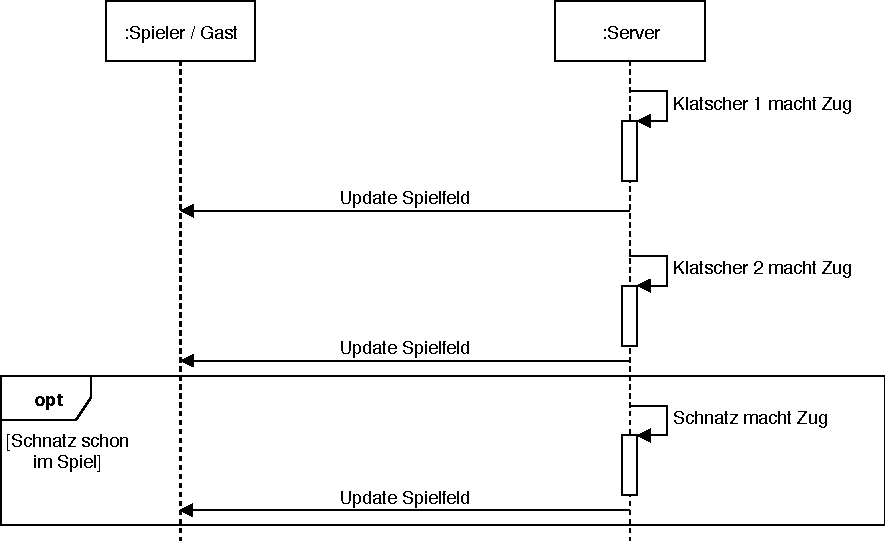
\includepdf[pages=-, scale=0.8, pagecommand={\subsubsection{Sequenzdiagramm Ballphase}}]{../Meilenstein02/images/SD_Ballphase.pdf}
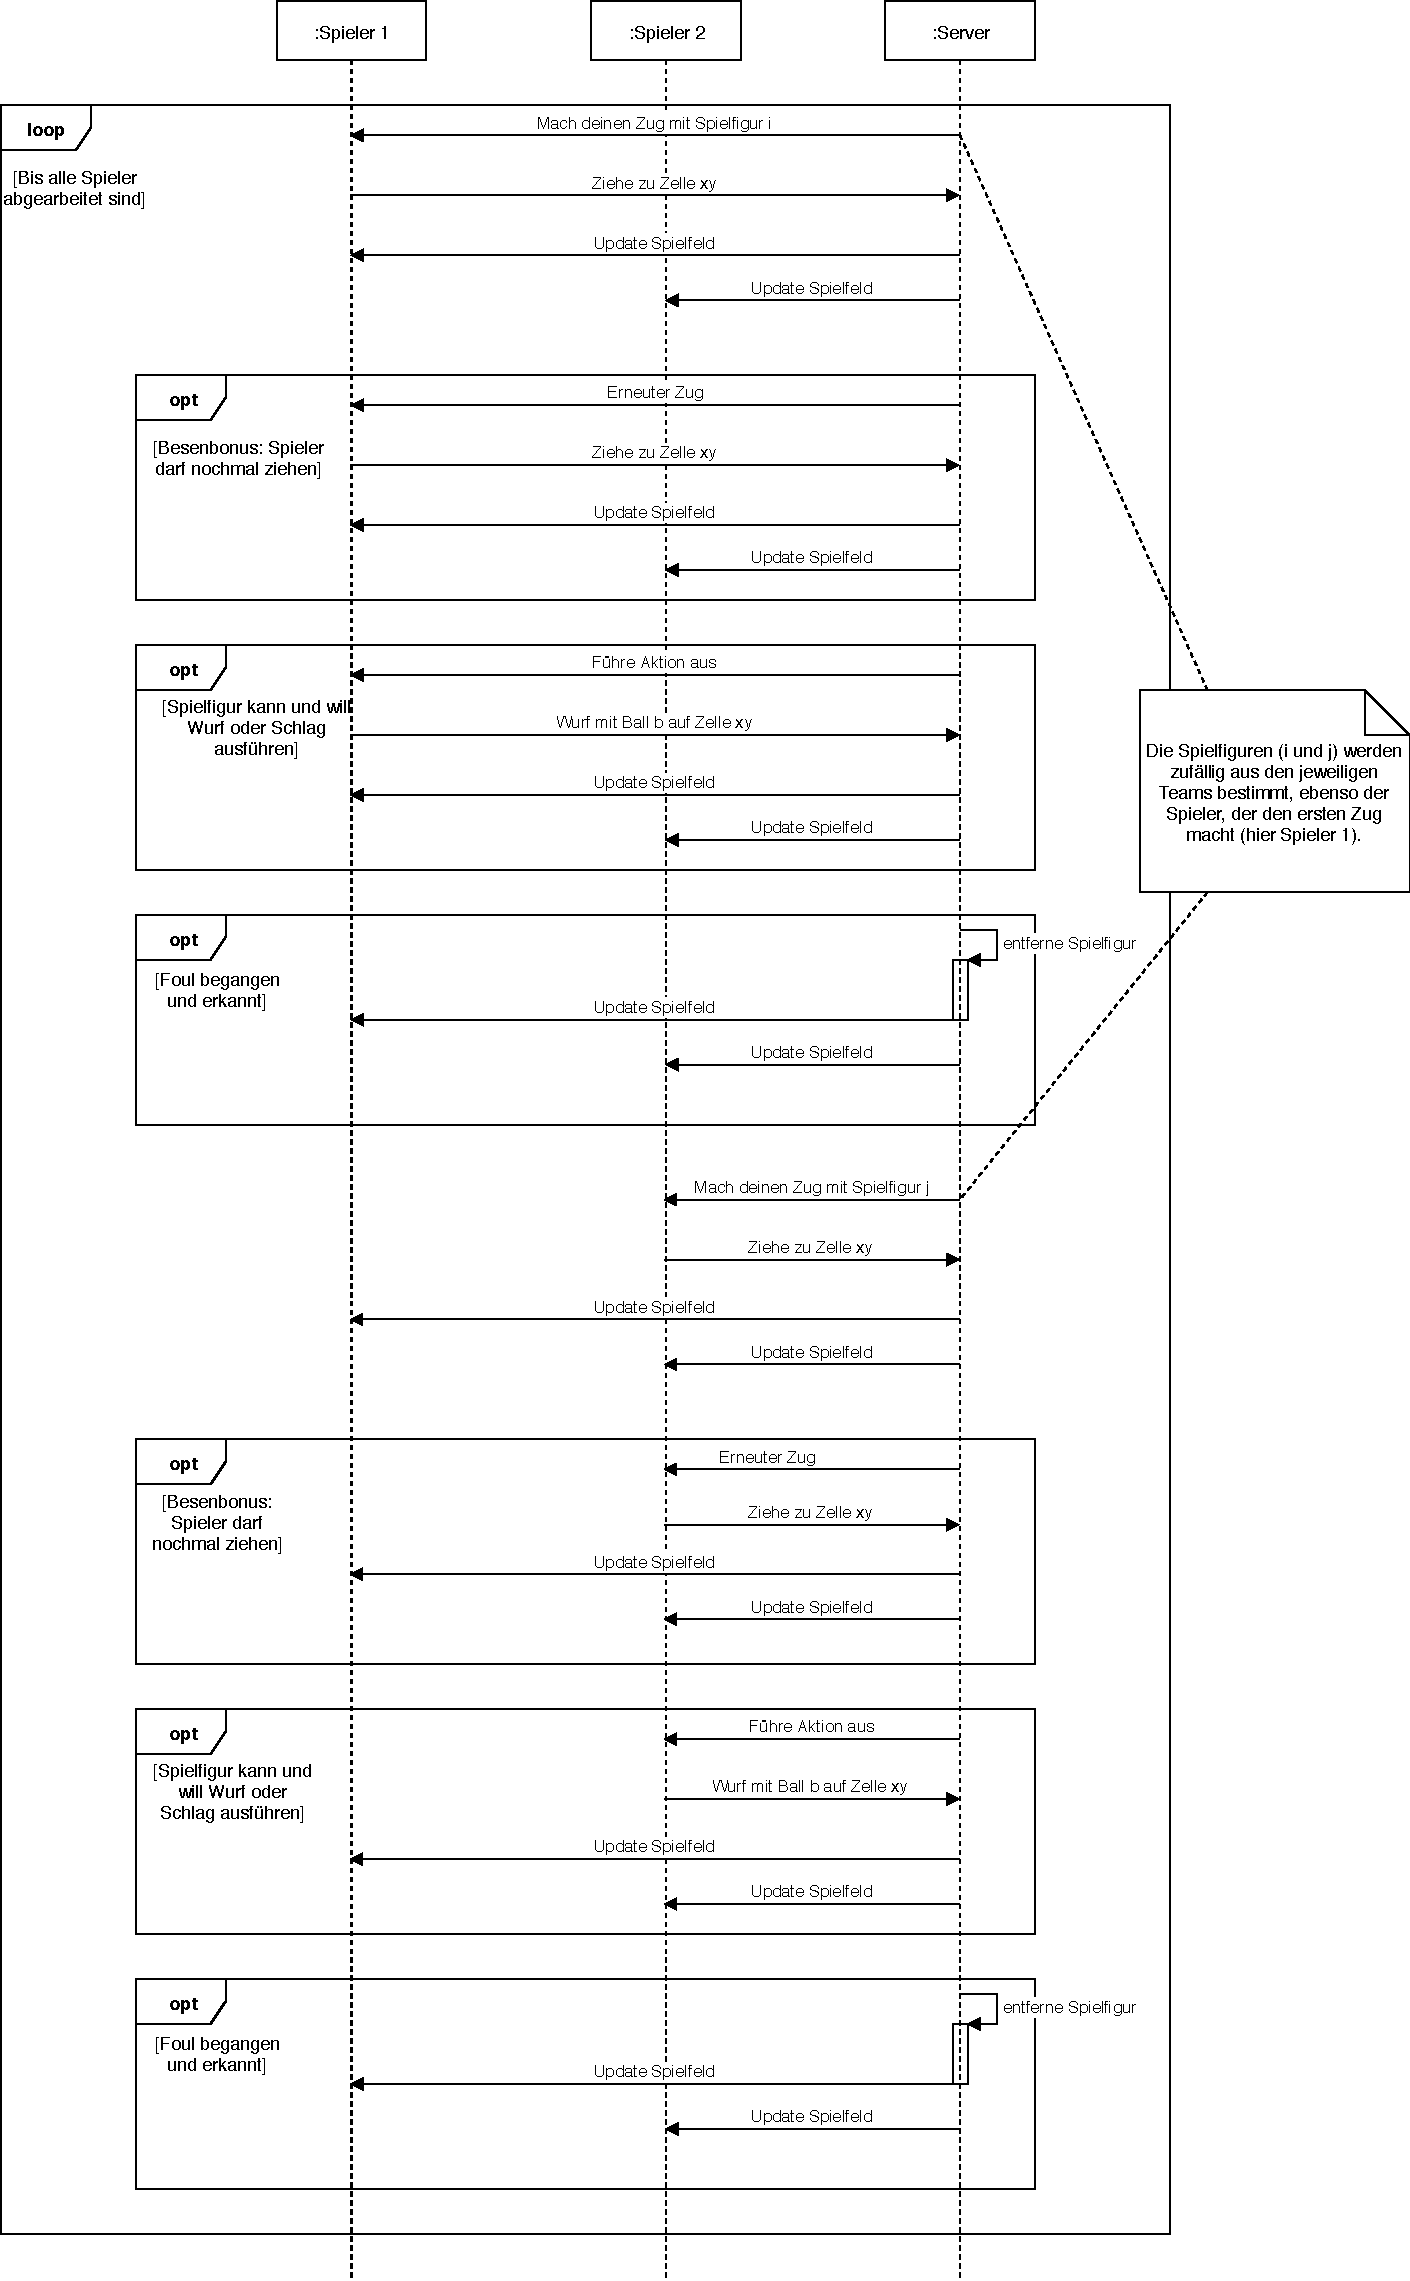
\includepdf[pages=-, scale=0.65, pagecommand={\subsubsection{Sequenzdiagramm Spielerphase}}]{../Meilenstein02/images/SD_Spielerphase.pdf}
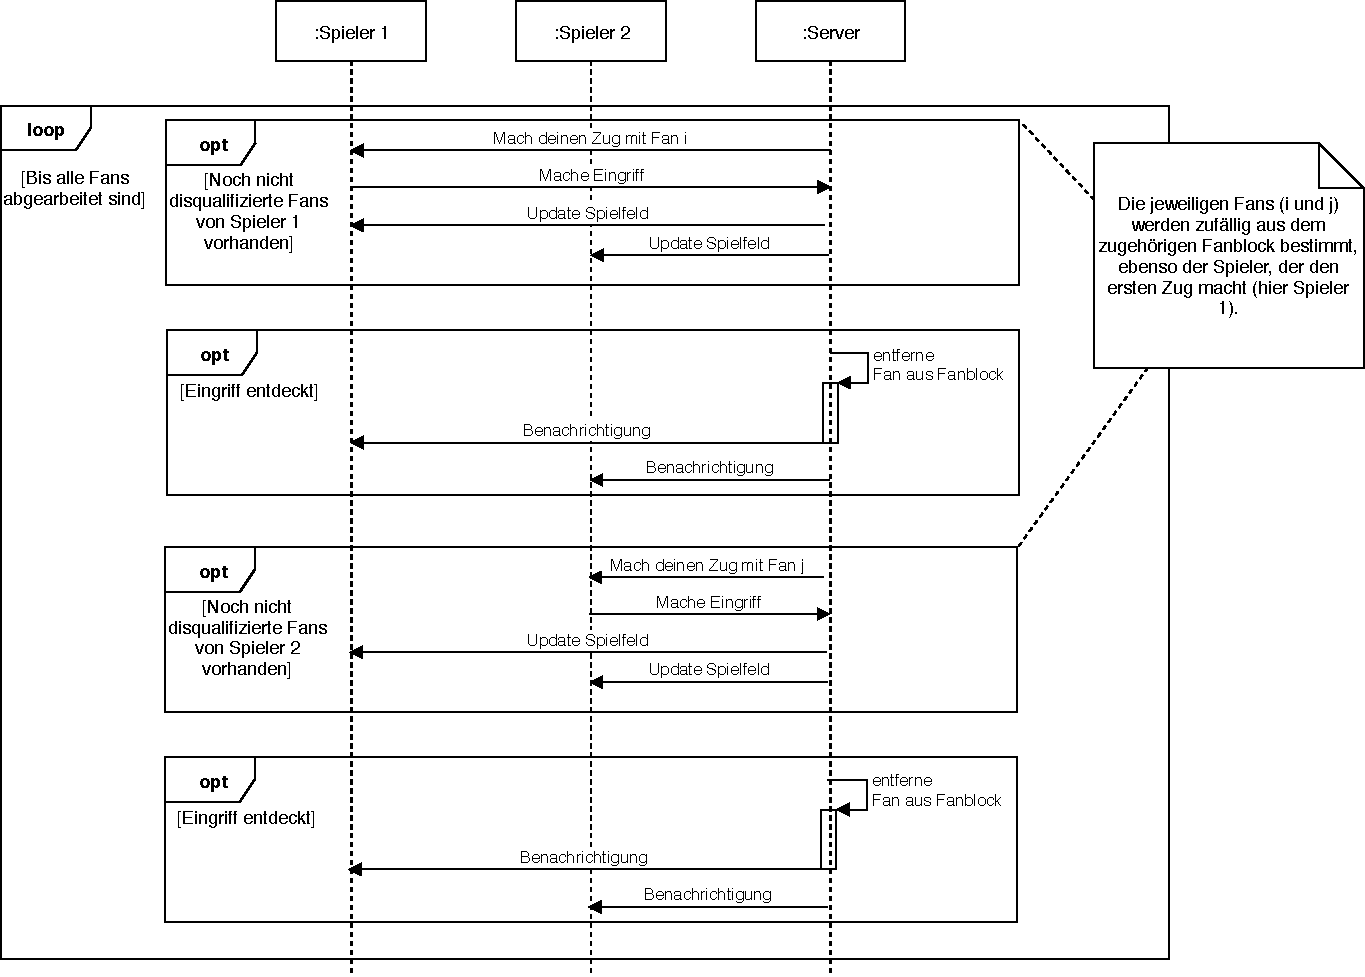
\includepdf[pages=-, scale=0.8, pagecommand={\subsubsection{Sequenzdiagramm Fanphase}}]{../Meilenstein02/images/SD_Fanphase.pdf}
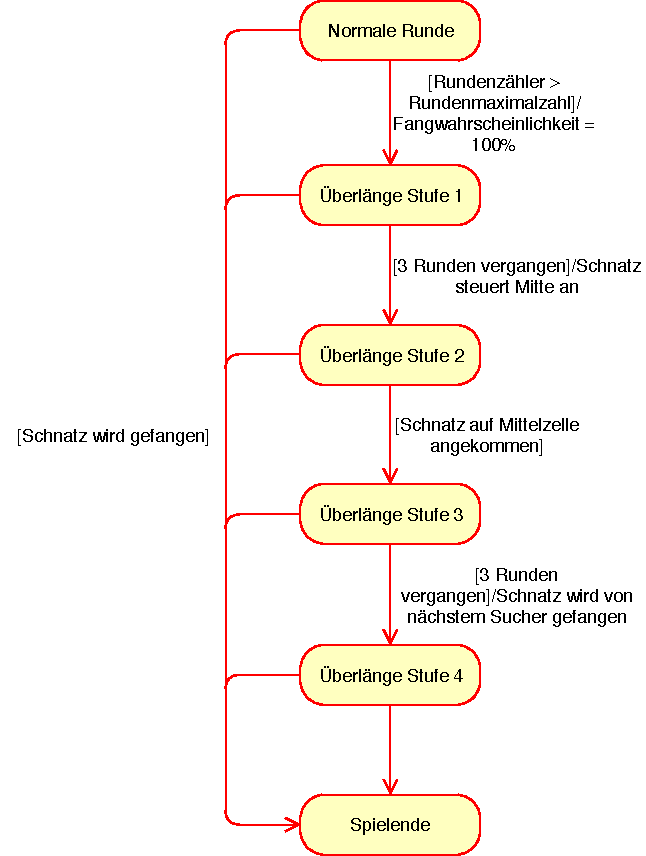
\includepdf[pages=-, scale=0.7, pagecommand={\subsubsection{State-Machine Überlängenbehandlung}}]{../Meilenstein02/images/SM_Ueberlaenge.pdf}
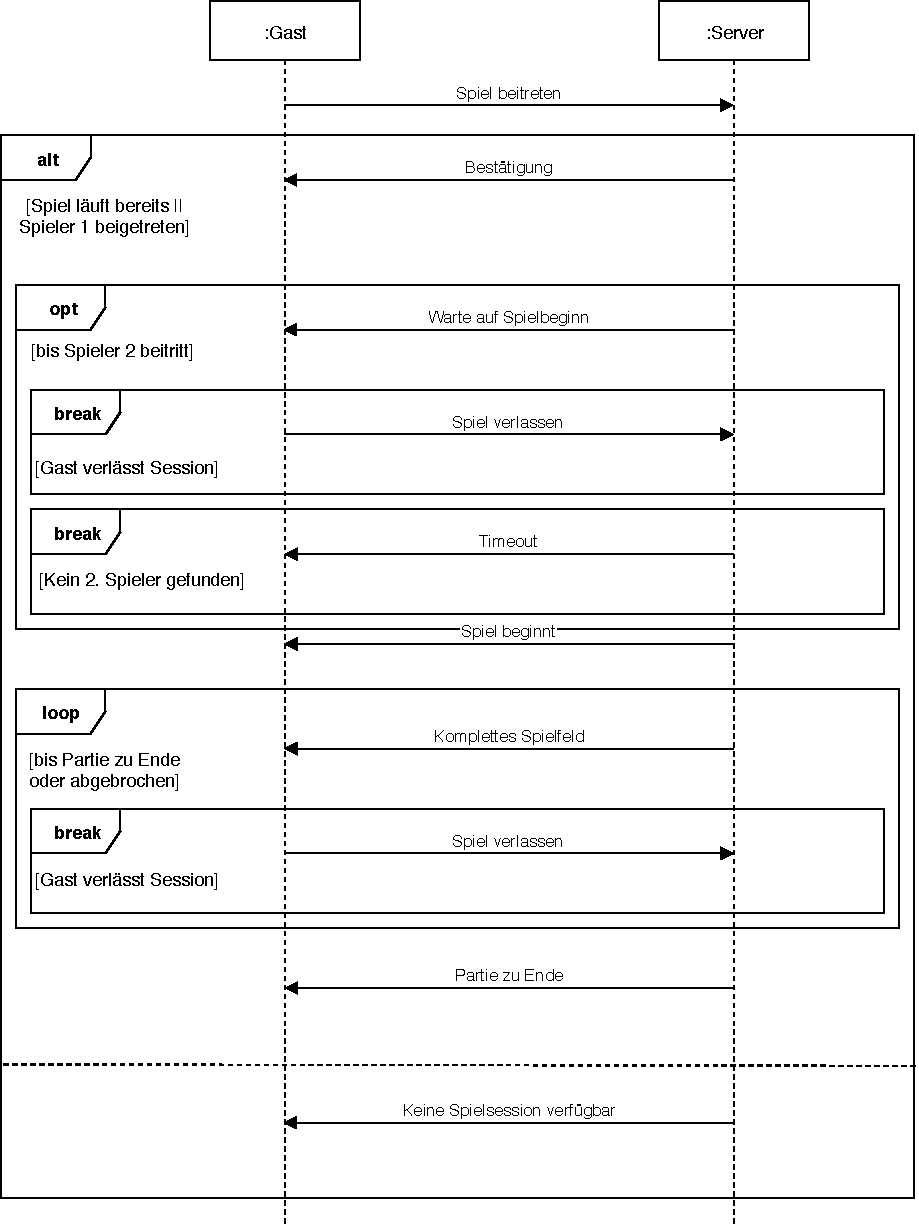
\includepdf[pages=-, scale=0.7, pagecommand={\subsubsection{Sequenzdiagramm Gast}}]{../Meilenstein02/images/SD_Gast.pdf}
